\usetikzlibrary{calc}
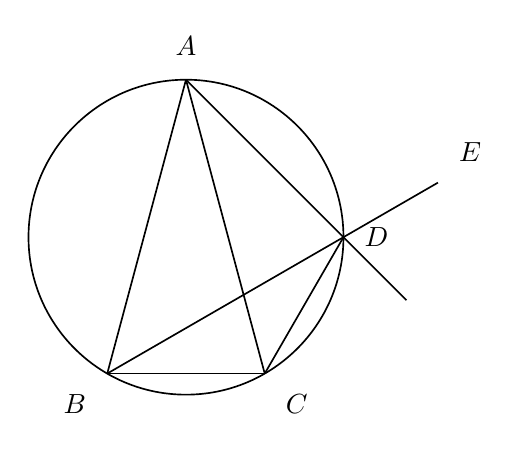
\begin{tikzpicture}[x=1cm,y=1cm,line width=.6pt,font=\normalsize]
\coordinate (O) at (0,0);
\coordinate (A) at (0,2);
\coordinate (B) at (-1,-1.7320508075688772);
\coordinate (C) at (1,-1.7320508075688772);
\coordinate (D) at (2,0);
\coordinate (E) at (3.2,0.6928203230275509);
\coordinate (F) at (2.8,-0.8);
\draw (O) circle[radius=2cm];
\draw (A)--(B);
\draw (B)--(C);
\draw (A)--(C);
\draw (A)--(D);
\draw (B)--(E);
\draw (C)--(D);
\draw (D)--(F);
\node[above=5pt] at (A) {$A$};
\node[below left=4pt] at (B) {$B$};
\node[below right=4pt] at (C) {$C$};
\node[right=4pt] at (D) {$D$};
\node[above right=4pt] at (E) {$E$};
\end{tikzpicture}
